\documentclass{seminar}
\usepackage{graphicx,color,fancybox,amsfonts,amsmath}
\usepackage[italian]{babel}
\usepackage{amsthm}
\usepackage{mathtools} %loads amsmath as well
\usepackage{wrapfig}

\theoremstyle{definition}
\newtheorem{definition}{Def.}

\newcommand{\RR}{\mathbb{R}}
\newcommand{\CC}{\mathbb{C}}
\newcommand{\PP}{\mathbb{P}}
\newcommand{\NN}{{\cal{N}}}
\newcommand{\bx}{\mathbf{x}}
\newcommand{\bmu}{\pmb{\mu}}
\newcommand{\brho}{\pmb{\rho}}
\newcommand{\balpha}{\pmb{\alpha}}
\newcommand{\bdelta}{\pmb{\delta}}
\newcommand{\btau}{\pmb{\tau}}
\newcommand{\bbeta}{\pmb{\beta}}

\def\bc{\begin{center}}
\def\ec{\end{center}}
\def\bs{\begin{slide}\begingroup\small}
\def\es{\endgroup\end{slide}}
\def\bg{\begingroup}
\def\eg{\endgroup}

\definecolor{greenf}{rgb}{.054, .5, .005}

\begin{document}
\large

\bs
\bc{\bf\color{blue}Tangent-based manifold approximation \\with locally linear models}\ec

\vskip 0.2in

\bc{{\color{red} Sofia Karygianni, Pascal Frossard}}\ec

\vskip 0.2in

\bc{\footnotesize \it Ecole Polytechnique Fédérale de Lausanne (EPFL), Signal Processing Laboratory (LTS4), CH-1015 Lausanne, Switzerland}\ec
\es

\bs
\bc{\bf\color{blue}introduzione}\ec
Motivati dal fatto che dati di dimensione alta siano comunemente difficili da trattare (The curse of dimensionality) si osserva che spesso segnali complessi possiedono una struttura sottostante che puo' permettere rappresentazioni adeguate in dimensione inferiore.
\vskip 0.2in
Un esempio e' dato da immagini catturate da diversi punti di vista di una stessa scena tridimensionale.
\es

\bs
\bc{\bf\color{blue}Nel dettaglio}\ec
In generale le varieta' (Manifold) sono strutture globalmente complesse che localmente ossia vicino ad ogni loro punto possiedono le stesse caratteristiche dello spazio Euclideo. In questo lavoro, si considerano varieta' $\it d$-dimensionali (differenziabili) immerse in uno spazio Euclideo di dimensione $\RR^{N}$ con $N \gg d$.
	Intuitivamente si puo' pensare a una varieta' d-dimensionale immersa in $\RR^{N}$ come alla generalizzazione di una superficie in $N$ dimensioni: un insieme di punti che localmente sembra vivere in $\RR^{d}$ ma che macroscopicamente sintetizza una struttura in $\RR^{N}$.
\vskip 0.2in
Un esempio classico sono una sfera in $\RR^{3}$ e una circonferenza in $\RR^{2}$ che sono rispettivamente due varieta' di dimensione $2$ e $1$.
\es

\bs
In questo lavoro si cerchera' di approssimare una varieta' arbitraria attraverso un modello semplice e computazionalmente efficiente ossia un set di sottospazi affini di dimensione arbitraria cercando di preservare globalmente la geometria della varieta'.


\begin{figure}[b]
\centering
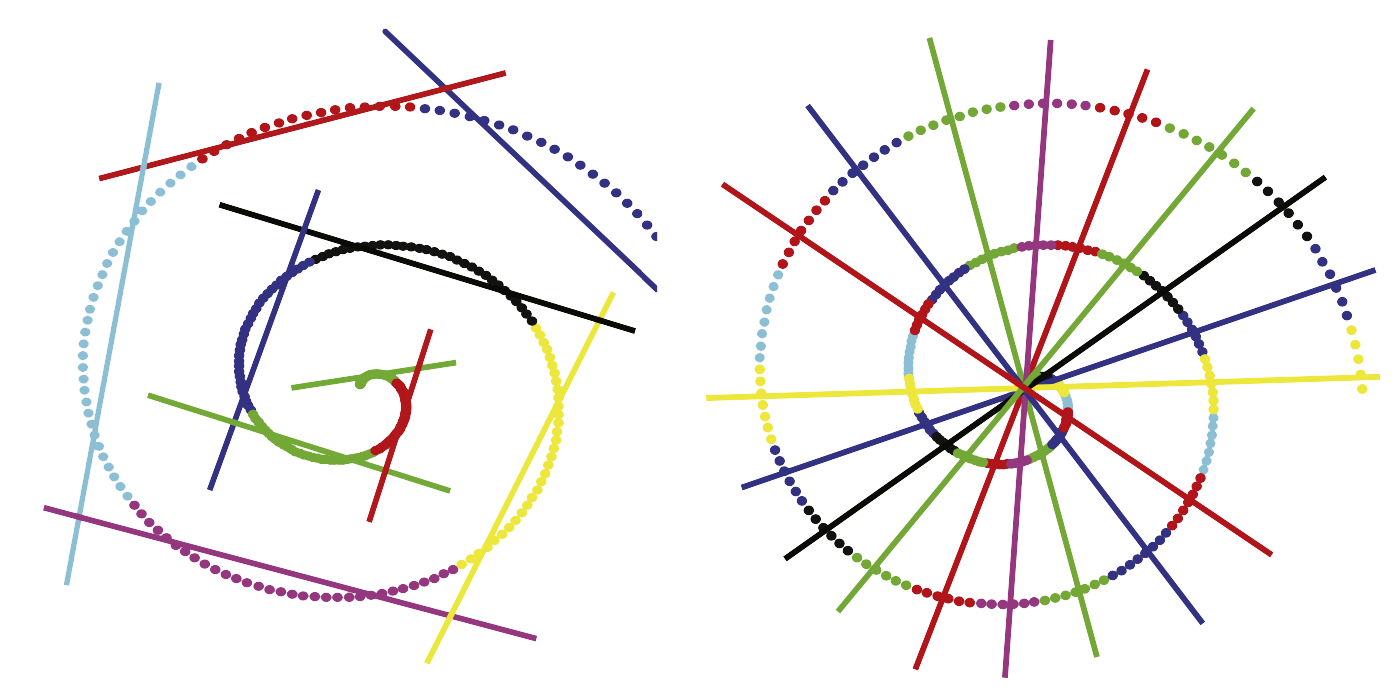
\includegraphics[width=0.7\textwidth]{goodandbadapprox.eps}
\caption{A sinistra una buona approssimazione di una varieta' 1D immersa in $\RR^{2}$ dove i colori rappresentano i diversi gruppi di punti approssimati da linee. A destra una cattiva approssimazione che non preserva la geometria della varieta'.}
\end{figure}
\es

\bs
\bc{\bf\color{blue}Framework}\ec
\begin{definition}[Varieta']
Un insieme $M\subseteq\RR^{N}$ e' detto varieta' differenziabile di dimensione $d$ se $\forall x\in M$ esiste un aperto $V\subseteq\RR^{N}$ t.c. $x\in V$ e un aperto $W\subseteq\RR^d$ ed esiste $f:W\to\RR^{N}$ iniettiva, differenziabile e ad inversa continua t.c.
\begin{itemize}
  \item $f(W)=M\cap V$ e
  \item $Rank(Df(y)) = d\ \forall y\in W$ (Dove $Df$ indica la Jacobiana di $f$)
\end{itemize}
\end{definition}
Supponiamo $f(a)=x$ allora la matrice $Df(a)$ e la corrispondente trasformazione lineare $f_{*}:\RR^{d}_{a}\to \RR^{N}_{x}$ definiscono un sottospazio di dimensione $d$ detto lo spazio tangente a $M$ in $x$ denotato $M_{x}$. \\
Per comodita' indicheremo da qui in poi con $M_x$ lo spazio tangente ad $M$ in $x$ traslato pero' all'origine di $\RR^N$.

\begin{figure}[b]
\centering
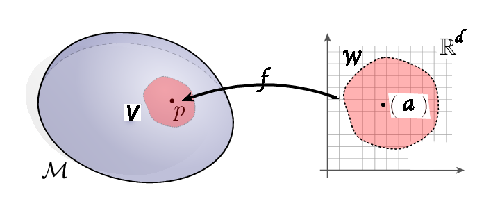
\includegraphics[width=0.5\textwidth]{manifold.eps}
\end{figure}
\es

\bs
\bc{\bf\color{blue}Osservazione motivante}\ec
E' fondamentale osservare che se per opportuni $x, V$ e $W \ f$ e' lineare allora $Df(a)=Df(b) \ \forall a, b\in W$ e dunque lo spazio tangente di tutti i punti in $M\cap V$ coincide (a meno di una traslazione) e la regione di spazio puo' essere perfettamente rappresentata con dei sottospazi affini.
Siamo allora interessati a determinare regioni dove la $\it{variazione}$ dello spazio tangente nei diversi punti e' bassa (cosi' $Df(a)\approx Df(b)$). \\
Definiamo dunque una metrica tra spazi tangenti.
\es

\bs
\bc{\bf\color{blue}Grassmann Manifold e Geodetiche}\ec
L'insieme dei sottospazi lineari di dimensione $d$ di $\RR^{N}$ e' detto Grassmanniana indicato $G_{N,d}(\RR^{N})$. In $G_{N,d}(\RR^{N})$ e' definita la distanza geodetica tra due sottospazi a partire dai loro angoli principali. In particolare possiamo definire la distanza tra $M_x$ e $M_y$ come

\begin{wrapfigure}{r}{0.4\textwidth}
    \centering
    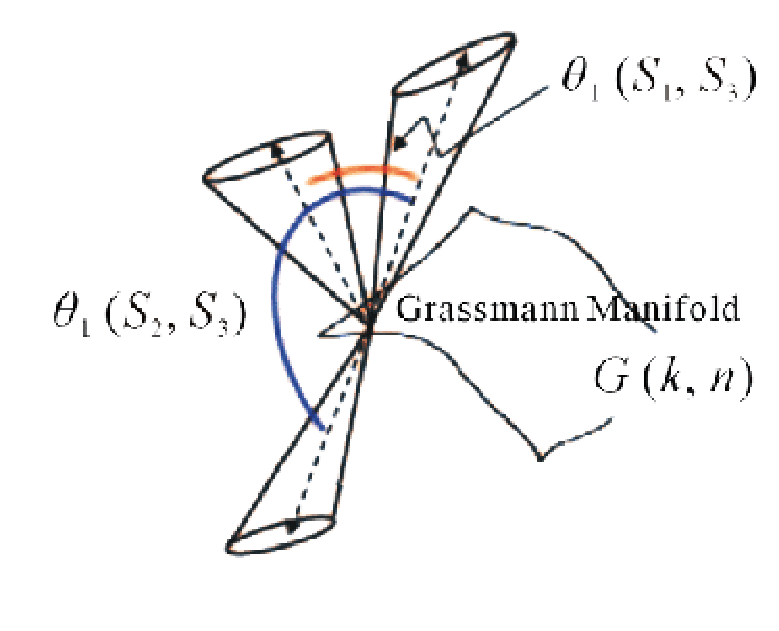
\includegraphics[width=0.4\textwidth]{principalangles.eps}
\end{wrapfigure}

\begin{equation*}
	D_{T}\left(M_{x}, M_{y}\right)=\left(\sum_{i=1}^{d} \theta_{i}^{2}\right)^{2}=\|\theta\|_{2}
\end{equation*}

dove $\theta=\left\{\theta_{1}, \ldots, \theta_{d}\right\}$ e' il vettore \\ degli angoli principali di $M_x$ e $M_y$. 
\es

\bs
\bc{\bf\color{blue}Punto medio di Karcher}\ec
Siamo inoltre interessati a poter calcolare una generalizzazione della media aritmetica applicata alla Grassmanniana.
\begin{definition}[Punto medio di Karcher su $G_{N,d}(\RR^{N})$ con distanza geodetica]
Il punto medio di un insieme $C$ di punti di $G_{N,d}(\RR^{N})$ rispetto alla distanza $D_T$ e' dato da
\begin{equation*}
M_{C}=\underset{M \in G_{N, d}}{\arg \min } \sum_{x \in C} D_{T}^{2}\left(M_{x}, M_{C_{i}}\right)
\end{equation*}
\end{definition}
Esistono vari metodi per risolvere in $M_C$ la precedente equazione, qui viene usata una formulazione data da $\it{J.M. Chang}$ che sfrutta la decomposizione in valori singolari (SVD).
\es

\bs
\bc{\bf\color{blue}Clustering}\ec
Sia $\mathcal{X} = \{x_k\in\RR^N, k\in [1, m]\}$ la rappresentazione di una varieta' attraverso un insieme di suoi punti. Sia $G_{\mathcal{X}}=G(\mathcal{X}, E)$ il grafo simmetrico non orientato che rappresenta la geometria della varieta'. Vogliamo determinare $\textbf{C}_{\mathcal{L}}=\{C_i, i\in [1, \mathcal{L}]\}$ partizione di $\mathcal{X}$ tale che $\forall i\ C_i$ possa essere ben rappresentato da un sottospazio affine che rispetti la geometria della varieta'.
\begin{definition}[Partizione]
$\textbf{C}_{\mathcal{L}}$ e' una partizione se $C_i\cap C_j = \emptyset \ \forall i\neq j, \ i,j\in \{1, ..., \mathcal{L} \}$ e $\bigcup_{i} C_i = \mathcal{X}$.
\end{definition}
Non tutte le partizione saranno pero' valide una condizione sufficiente e' che la partizione sia formata solo da cluster con sottografi connessi.
\begin{definition}[Sottografo connesso]
Dato $G_{C_i}=G(C_i, E_i)$ sottografo dove $E_i=\{a_{ij}\in E: \ x_i, x_j\in C_i\}$ diciamo che esso e' connesso se ogni coppia di nodi $x_i, x_j\in C_i$ e' connessa.
\end{definition}
\es

\bs
\bc{\bf\color{blue}Validita'}\ec
Denotiamo l'insieme delle partizioni valide $\Phi_\mathcal{L}(\mathcal{X})$.
\begin{definition}[Predicato di $\it{validita'}$]
$\Phi_\mathcal{X}(\textbf{C}_\mathcal{L}) \equiv \textbf{C}_\mathcal{L}\in \Phi_\mathcal{L}(\mathcal{X})$ definito come
\begin{equation*}
\begin{gathered}
\Phi_\mathcal{X}(\textbf{C}_\mathcal{L}) = \bigwedge_{C_i\in\textbf{C}_\mathcal{L}}\phi(C_i) \\
\phi(C_i) = 
  \begin{cases}
                                   Vero & \text{Se $C_i$ e' connesso} \\
                                   Falso & \text{altrimenti} \\
  \end{cases}
\end{gathered}
\end{equation*}
\end{definition}
\bc{\bf\color{blue}Fondibilita'}\ec
Possiamo definire anche un predicato di fondibilita' $\Psi$ che descrive se due cluster possono essere uniti dando vita a una partizione ancora valida, i predicati di fondibilita' e validita' sono legati dalla relazione seguente: \\
Se $C_i,C_j\neq \emptyset, C_i\cap C_j =\emptyset, \ \phi(C_i)\wedge\phi(C_j)$ e $\Psi(C_i, C_j) \implies \phi(C_i\cup C_j)$
Evitando una definizione formale, due cluster saranno fondibili se esiste un $\it{edge}$ che li collega.
\es

\bs
\begin{figure}[t]
\centering
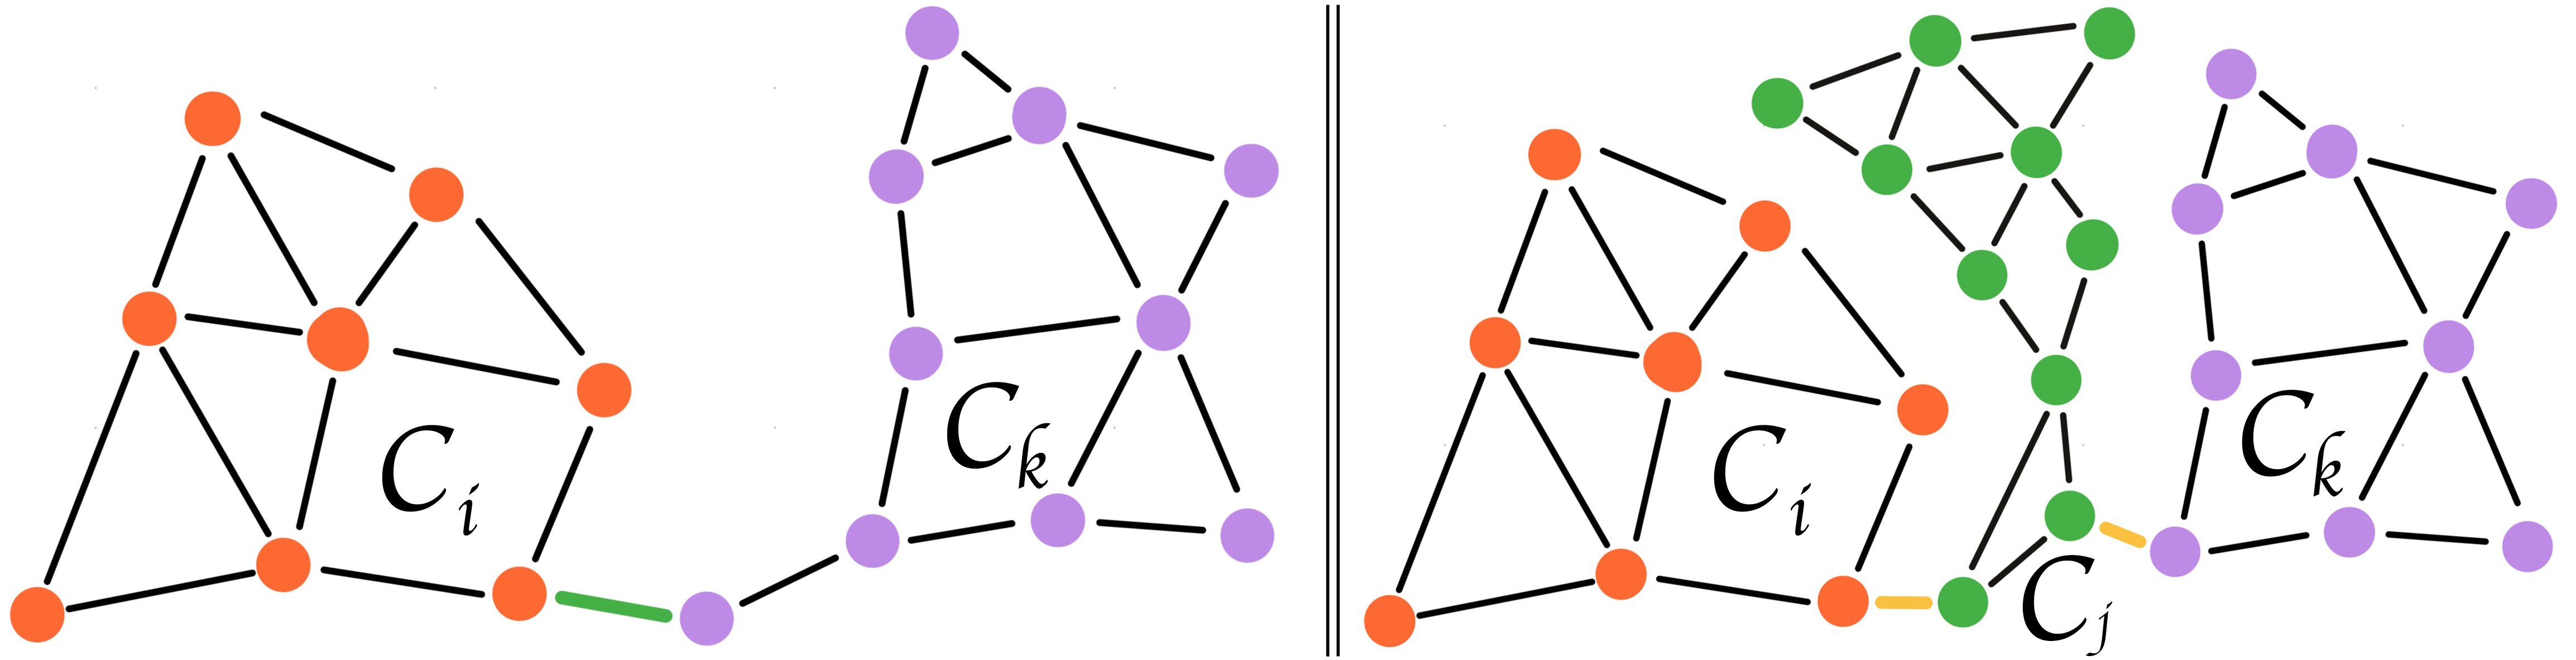
\includegraphics[width=1\textwidth]{connectedclusters.eps}
\caption{A sinistra due cluster $C_i$ e $C_k$ connessi e dunque fondibili. A destra tre cluster dove sia $C_i$ che $C_k$ sono fondibili con $C_j$ ma $C_i$ e $C_k$ non sono fondibili. \\
E' facile osservare che fondendo le coppie (fondibili) in entrambe le configurazioni la partizione risultante e' composta da sottografi connessi e dunque valida.}
\end{figure}
\es

\bs
\bc{\bf\color{blue}Bonta' di una partizione}\ec
Cerchiamo ora una funzione $\mathcal{P}$ che valuti la bonta' di una partizione, definiamo
\begin{equation*}
\begin{gathered}
	\mathcal{P}(\textbf{C}) = \sum_{C_i\in\textbf{C}}p(C_i) \ \ \text{con} \\
	p(C_i) = \sum_{x\in C_i}D^{2}_T(M_{C_i}, M_x)
\end{gathered}
\end{equation*}
Osserviamo che per definizione $\mathcal{P}$ e' distributiva sui cluster e non negativa, inoltre e' nulla sui cluster formati da singoletti.
\es

\end{document}
